\newpage
\section{Olaf Grykalowksi}
\label{PlaFon}

I added a photo which spit some truth (see Figure~\ref{fig:god}).

\begin{meme}
    \centering
    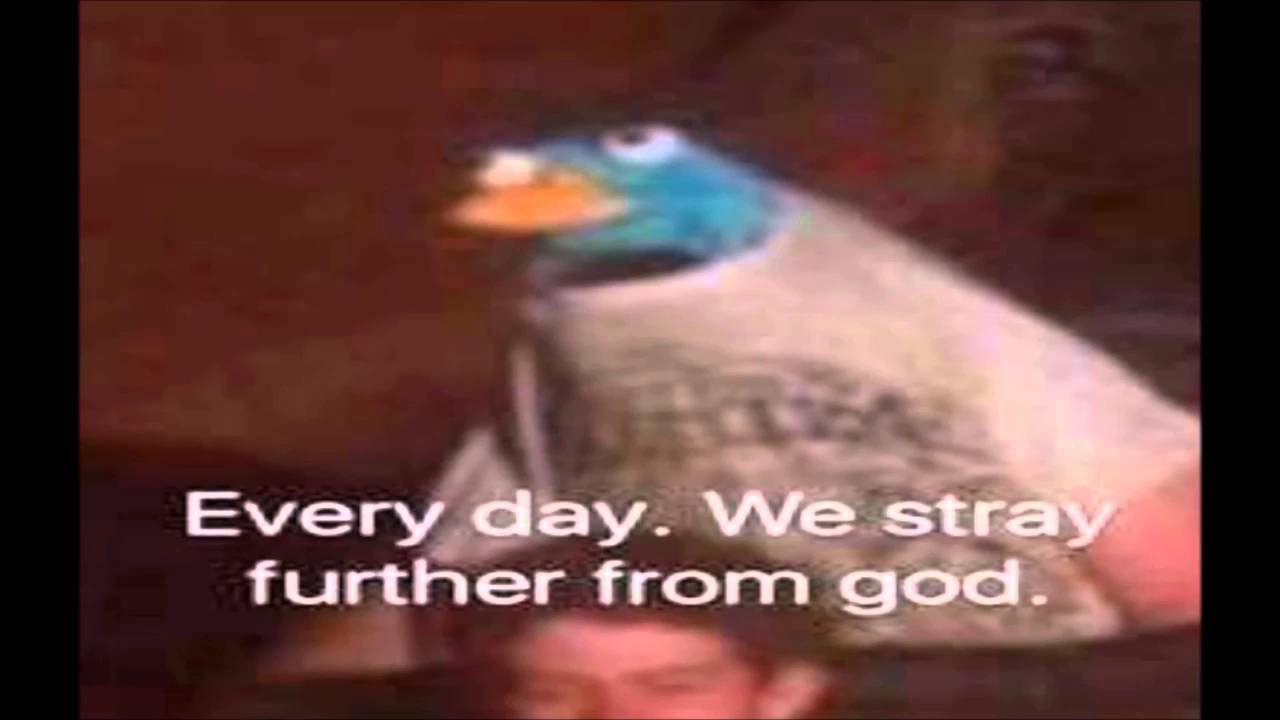
\includegraphics[width=0.8\textwidth]{pictures/god.jpg}
    \begin{center}
    \caption{This is my favorite meme.}
    \end{center}
    \label{fig:god}
\end{meme}

\begin{math}

I added some math equation:\newline
    
    H = -\sum p(x) log p(x) \newline
    
    A = \pi r^2 + \frac{1}{2}
    \\
\end{math}
\\
I added unordered list: \\
\newline
List of books:
\begin{itemize}

    \item[$\blacksquare$] The way of supiroir man 
    \item[$\blacksquare$] Why we sleep 
    \item[$\blacksquare$] How to win friends and influence people
    \item[$\blacksquare$] Unscripted
    
\end{itemize}

\newline
I added ordered list: 
\begin{enumerate}
    \item The way of supiroir man 
    \item Why we sleep 
    \item How to win friends and influence people
    \item Unscripted
\end{enumerate}


Table ~\ref{tab:trigonometry_table} represents trigonometry table. 
\begin{table}[htbp]
\centering
\begin{tabular}{
>{\columncolor[HTML]{38761d}}c 
>{\columncolor[HTML]{FFFFFF}}c 
>{\columncolor[HTML]{FFFFFF}}c 
>{\columncolor[HTML]{FFFFFF}}c 
>{\columncolor[HTML]{FFFFFF}}c l}
\cellcolor[HTML]{04ee51} rand() & \cellcolor[HTML]{04ee512} a & \cellcolor[HTML]{04ee51}b & \cellcolor[HTML]{04ee51}c & \cellcolor[HTML]{04ee51}d &  \\
1 & 6      & 9      & 3      & 2 &  \\
2 & 51 & 16 & 69 & 39        &  \\
3 & 855 & 359 & 574 & 567      &  \\
4° & 5278 & 8021 & 4563 & 5130      &  \\
5° & 73136 & 78783 & 75852 & 32654      &  \\


\end{tabular}
\label{tab:rand_table}
\caption{This is a table}
\end{table}


\begin{center}
\textbf{One Summer Night}\\
\underline{\emph{The fact that Henry Armstrong}}  was buried did not seem to him to prove that he was dead: he had always been a hard man to convince. That he really was buried, the testimony of his senses compelled him to admit.\par 
His posture -- flat upon his back, with his hands crossed upon his stomach and tied with something that he easily broke without profitably altering the situation -- the strict confinement of his entire person, the black darkness and profound silence, made a body of evidence impossible to controvert and he accepted it without \small{cavil}. \par
\textit{to be continued}
\end{center}




